\documentclass[a4paper,12pt]{scrartcl}
\usepackage{xcolor}
\usepackage[UKenglish]{isodate}%http://ctan.org/pkg/isodate
\usepackage[a4paper,left=2cm, right=2cm,top=2.7cm, bottom=3cm]{geometry}
\usepackage{changepage}
\usepackage{fancyhdr}
\usepackage[export]{adjustbox}
\usepackage{sectsty}
\usepackage[titles]{tocloft}
\usepackage{hyperref}
\usepackage{graphicx}
\hypersetup{
    colorlinks,
    citecolor=black,
    filecolor=black,
    linkcolor=black,
    urlcolor=black
}

\hyphenchar\font=-1
\setlength{\cftbeforesecskip}{4pt}

\newenvironment{subs}
{\adjustwidth{3em}{0pt}}
{\endadjustwidth}
\renewcommand{\cftsecleader}{\cftdotfill{\cftdotsep}}
\renewcommand{\familydefault}{\sfdefault}

\pagestyle{fancy}
\fancyhf{}
\renewcommand{\headrulewidth}{0pt}
\lhead{\today}
\chead{System Design Document}
\rhead{\ProjectName}
\lfoot{
\includegraphics[scale=0.147,valign=c]{EIST.png}}
\cfoot{\thepage}
\rfoot{
\includegraphics[scale=0.4,valign=c]{TUM.png}}

\newcommand{\ProjectName}{TUM Social}

\begin{document}
    \section*{Purpose}
    The system design is documented in the System Design Document (SDD). It describes additional design goals set by the software architect, the subsystem decomposition (with UML class diagrams), hardware/software mapping (with UML deployment diagrams), data management, access control, control flow mechanisms, and boundary conditions. The SDD serves as the binding reference document when architecture-level decisions need to be revisited.

    \section*{Audience}
    The audience for the SDD includes the system architect and the object designers as well as the project manager.
    \nopagebreak

    \renewcommand{\contentsname}{Table of Contents}
    \tableofcontents
    \section*{Document History}

    \begin{tabular}{
        |p{\dimexpr.08\linewidth-2\tabcolsep-1.3333\arrayrulewidth}% column 1
        |p{\dimexpr.17\linewidth-2\tabcolsep-1.3333\arrayrulewidth}% column 2
        |p{\dimexpr.20\linewidth-2\tabcolsep-1.3333\arrayrulewidth}
        |p{\dimexpr.56\linewidth-2\tabcolsep-1.3333\arrayrulewidth}|% column 3
    }
        \hline
        Rev. & Author & Date            & Changes          \\
        \hline
        1    & name   & 31st April 2022 & Sample changes 1 \\
        \hline
        2    & name   & 15th May 2022   & Sample changes 1 \\
        \hline
        3    & name   & 29th May 2022   & Sample changes 1 \\
        \hline
        4    & name   & 12th June 2022  & Sample changes 1 \\
        \hline
        5    & name   & 26th June 2022  & Sample changes 1 \\
        \hline
    \end{tabular}
    \newpage
    \sectionfont{\color[HTML]{355a8a}}  % sets colour of chapters
    \subsectionfont{\color[HTML]{4e81bc}}


    \section{Introduction}
    The purpose of the Introduction is to provide a brief overview of the software architecture. It also provides references to other documents.
    \begin{subs}
        \subsection{Overview}
        They system is made up of controllers that 

        \subsection{Definitions, acronyms, and abbreviations}

        \subsection{References}
    \end{subs}


    \section{Design Goals}
    This section describes the design goals and their prioritization (e.g. usability over extensibility). These are additional nonfunctional requirements that are of interest to the developers. Any trade-offs between design goals (e.g., usability vs. functionality, build vs. buy, memory space vs. response time), and the rationale behind the specific solution should be described in this section. Also the rationale of all other decisions must be consistent with described design goals.
    
    When designing the system we had certain non-functional requirements in mind. We determined the most important of these to be scalability, usability and maintainablility. These fundamental priciples shaped the development of our system and are easily noticed by users. Our registration process is very simple and new users can sign up with just a couple clicks and have full access to all the features right away. Furthermore, the database is highly capable and enables the network to expand and support a growing number of users. The code is also easy to read as the system uses the MVC pattern with various different controllers for different features.


    \section{Subsystem Decomposition}
    This section describes the decomposition of the system into subsystems and the services provided by each subsystem. The services are the seed for the APIs detailed in the Object Design Document. The system can generally be seperated into 3 distinct components. The database, server and client. The database stores all data and offers a facade interface to let the server request data. The server is a standard spring boot application, which handles all of the clients requests. The client provides the end user with a GUI, that makes use of various controllers for different functions, to make requests from the server. The following diagram is a rough representation of the system seperated into its basic components/subsystems.
    	
    	
        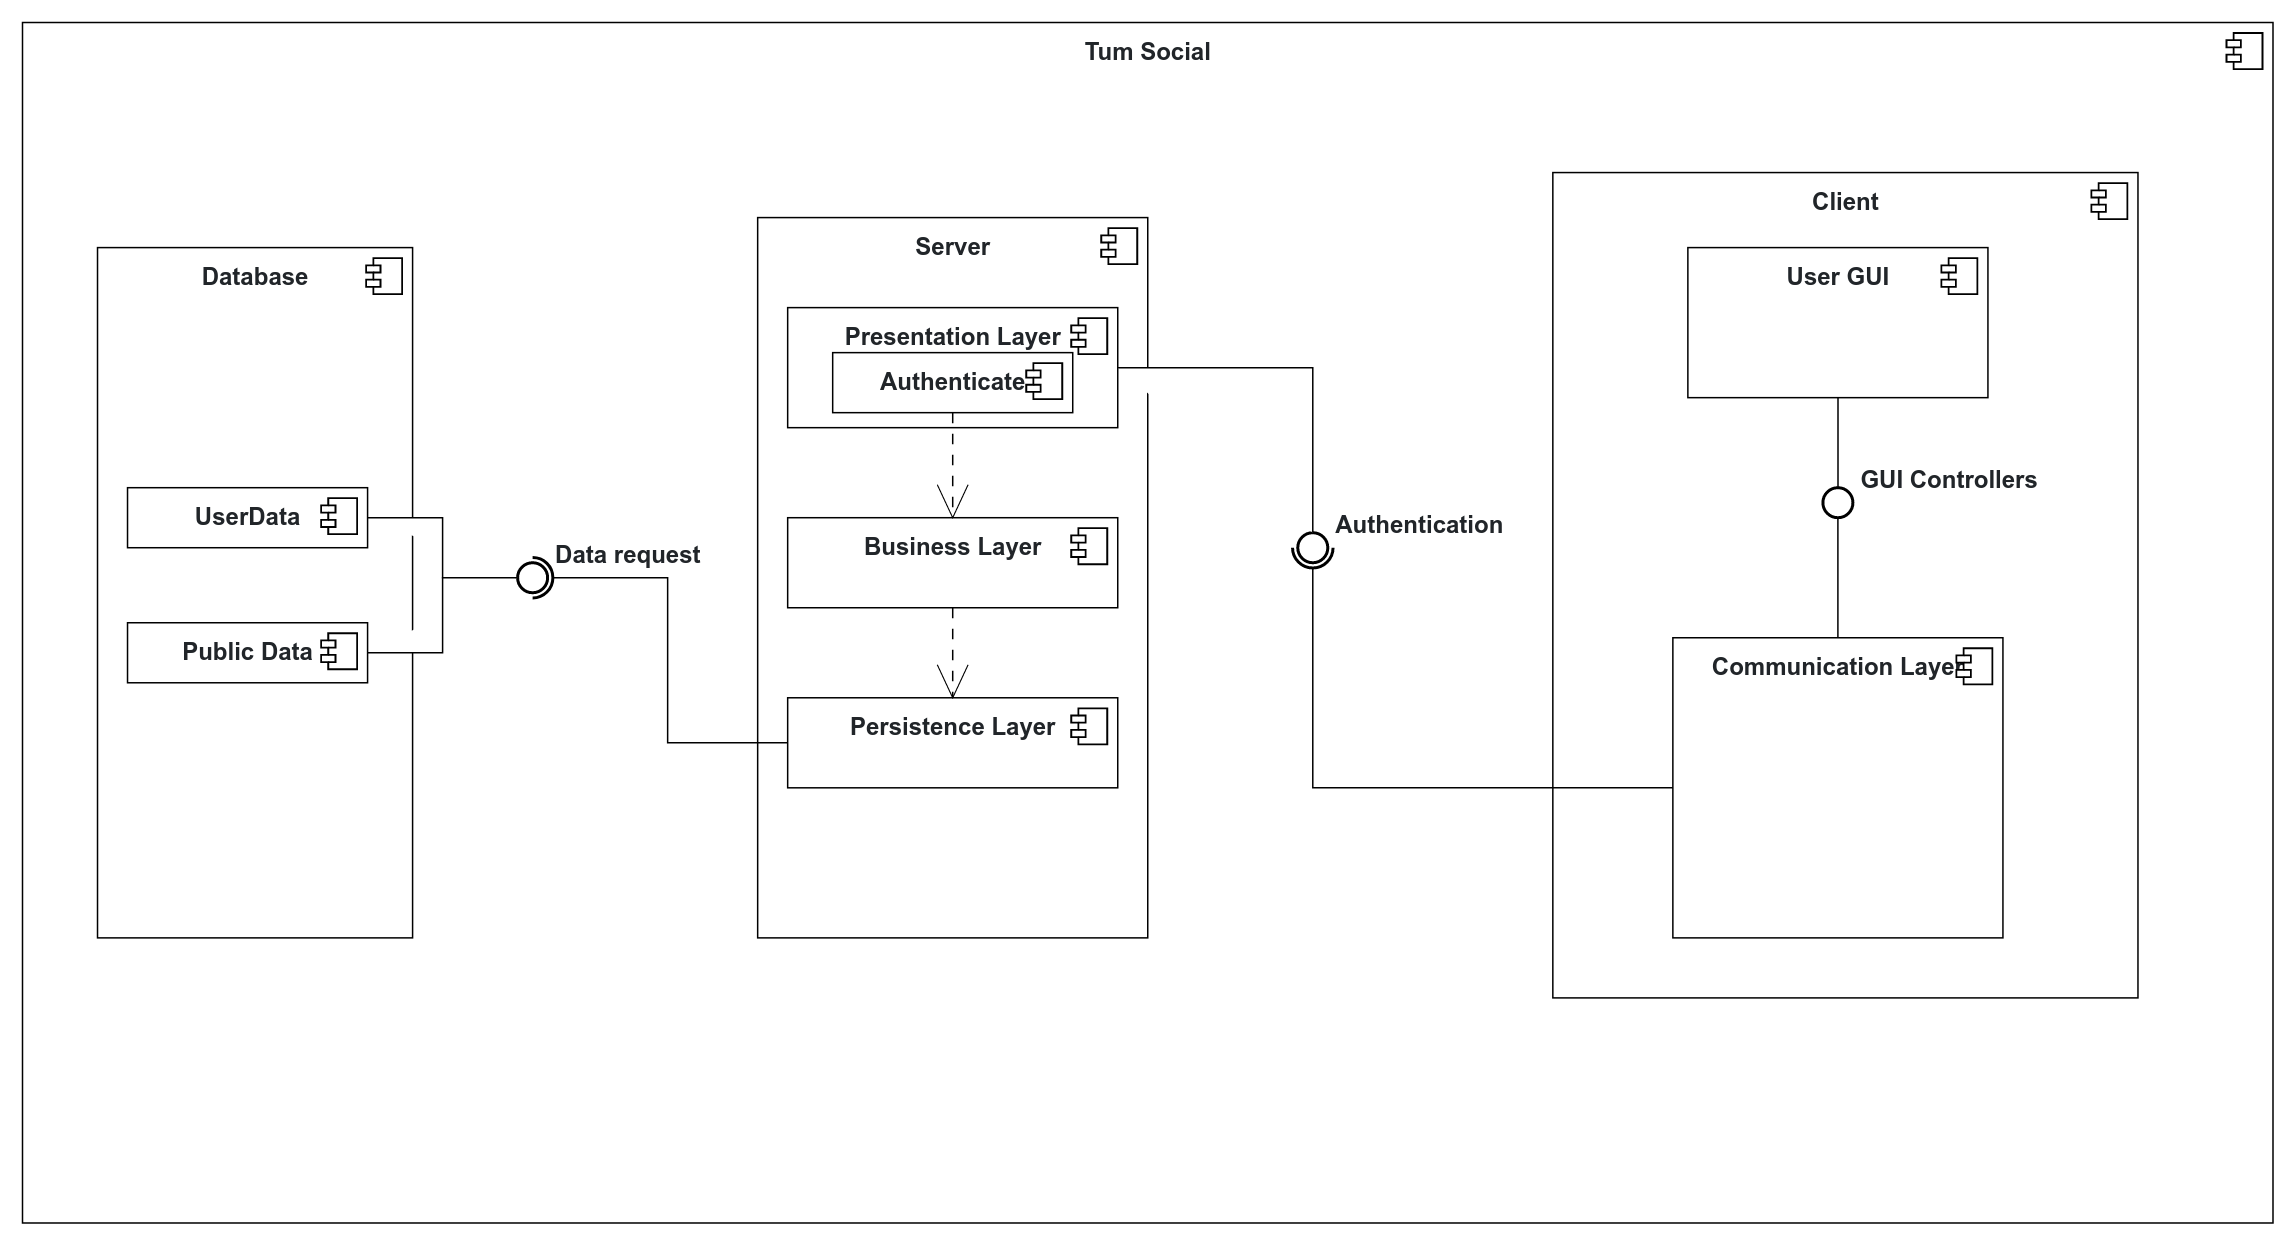
\includegraphics[scale=0.15]{ComponentDiagram.png}
  


    \section{Hardware/Software Mapping}
    This section describes how the subsystems are mapped onto existing hardware and software components. A UML deployment diagram accompanies the description. The existing components are often off-the-shelf components. If the components are distributed on different nodes, the network infrastructure and the protocols are also described.


    \section{Persistent Data Management}
    This section describes how the entity objects are mapped to persistent storage.
    It contains a rationale of the selected storage scheme, file system or database, a description of the selected database and database administration issues.


    \section{Access Control and Security}
    This section describes the access control and security issues based on the nonfunctional requirements in the requirements analysis document. It also describes the implementation of the access matrix based on capabilities or access control lists, the selection of authentication mechanisms and the use of encryption algorithms.


    \section{Global Software Control}
    This section describes the control flow of the system, in particular, whether a monolithic, event-driven control flow or concurrent processes have been selected, how requests are initiated and specific synchronisation issues.


    \section{Boundary Conditions}
    This section describes the use cases how to start up the separate components of the system, how to shut them down, and what to do if a component or the system fails. \\First of all the serer needs to be started, as it handles all of the communication within the network. When the server is running clients can start up and try to connect to it. If a connection cannot be successfully made, clients will simply have to retry until the server responds. Ideally the server is running continously, but it is possible that the server as somepoint stops answering requests. This may be because of a "distributed denia-of-service" attack or technical problems. When this happens the clients will not be able to communicate with each other. All connected clients will experience a lack of response from the server. The clients will have to wait until the server is operational again. If at some point the system is supposed to shut sown indefinitly, the clients should end the connection with the server before it will shutdown. 

\end{document}
